The model files are written in the syntax of DYNARE and have a common structure.
As an example we take the simple New-Keynesian model by \cite{RotembergWoodford1997} to
explain the structure of the mod-files, its model specific parts and the common model data base blocks. The current example is based on the DYNARE 4.5.6 version of the Modelbase. The mod-file is shown in {\bf Figure \ref{img:modStructureRW97a}} and {\bf Figure \ref{img:modStructureRW97b}}. However, the explanations apply to all models.
In the following, the two main parts of a mod-file, the preamble and the model block, are described step by step.

\begin{figure}[H]
\centering
\caption{\textsc{Structure of the model files: The Preamble}}
\vspace{0.2cm}
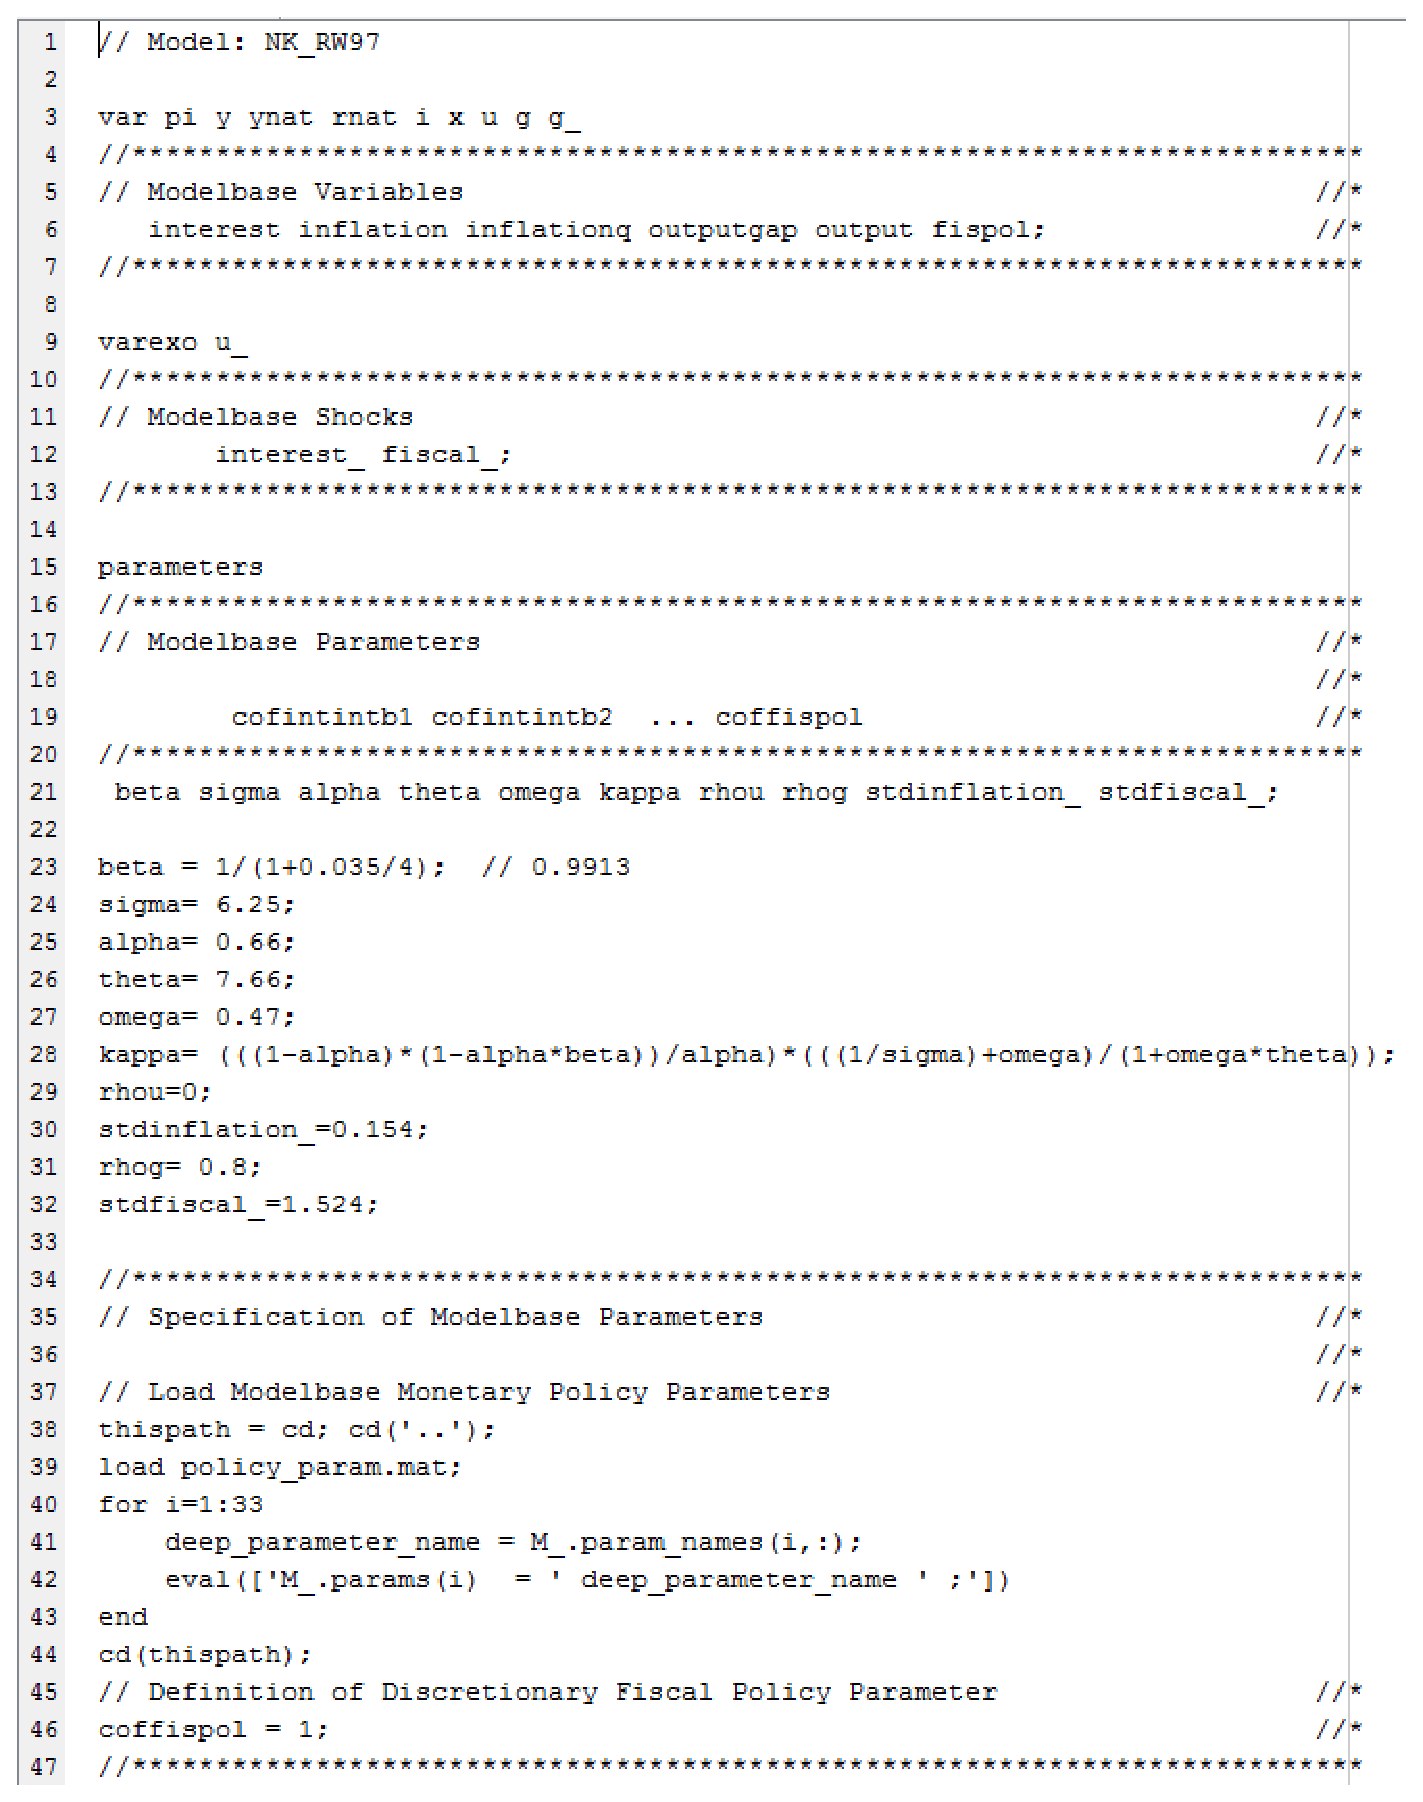
\includegraphics[width=15cm,keepaspectratio]{modStructureRW97a.eps}\\
\label{img:modStructureRW97a}
\end{figure}

\begin{figure}[H]
\centering
\caption{\textsc{Structure of the model files: The Model Block}}
\vspace{0.2cm}
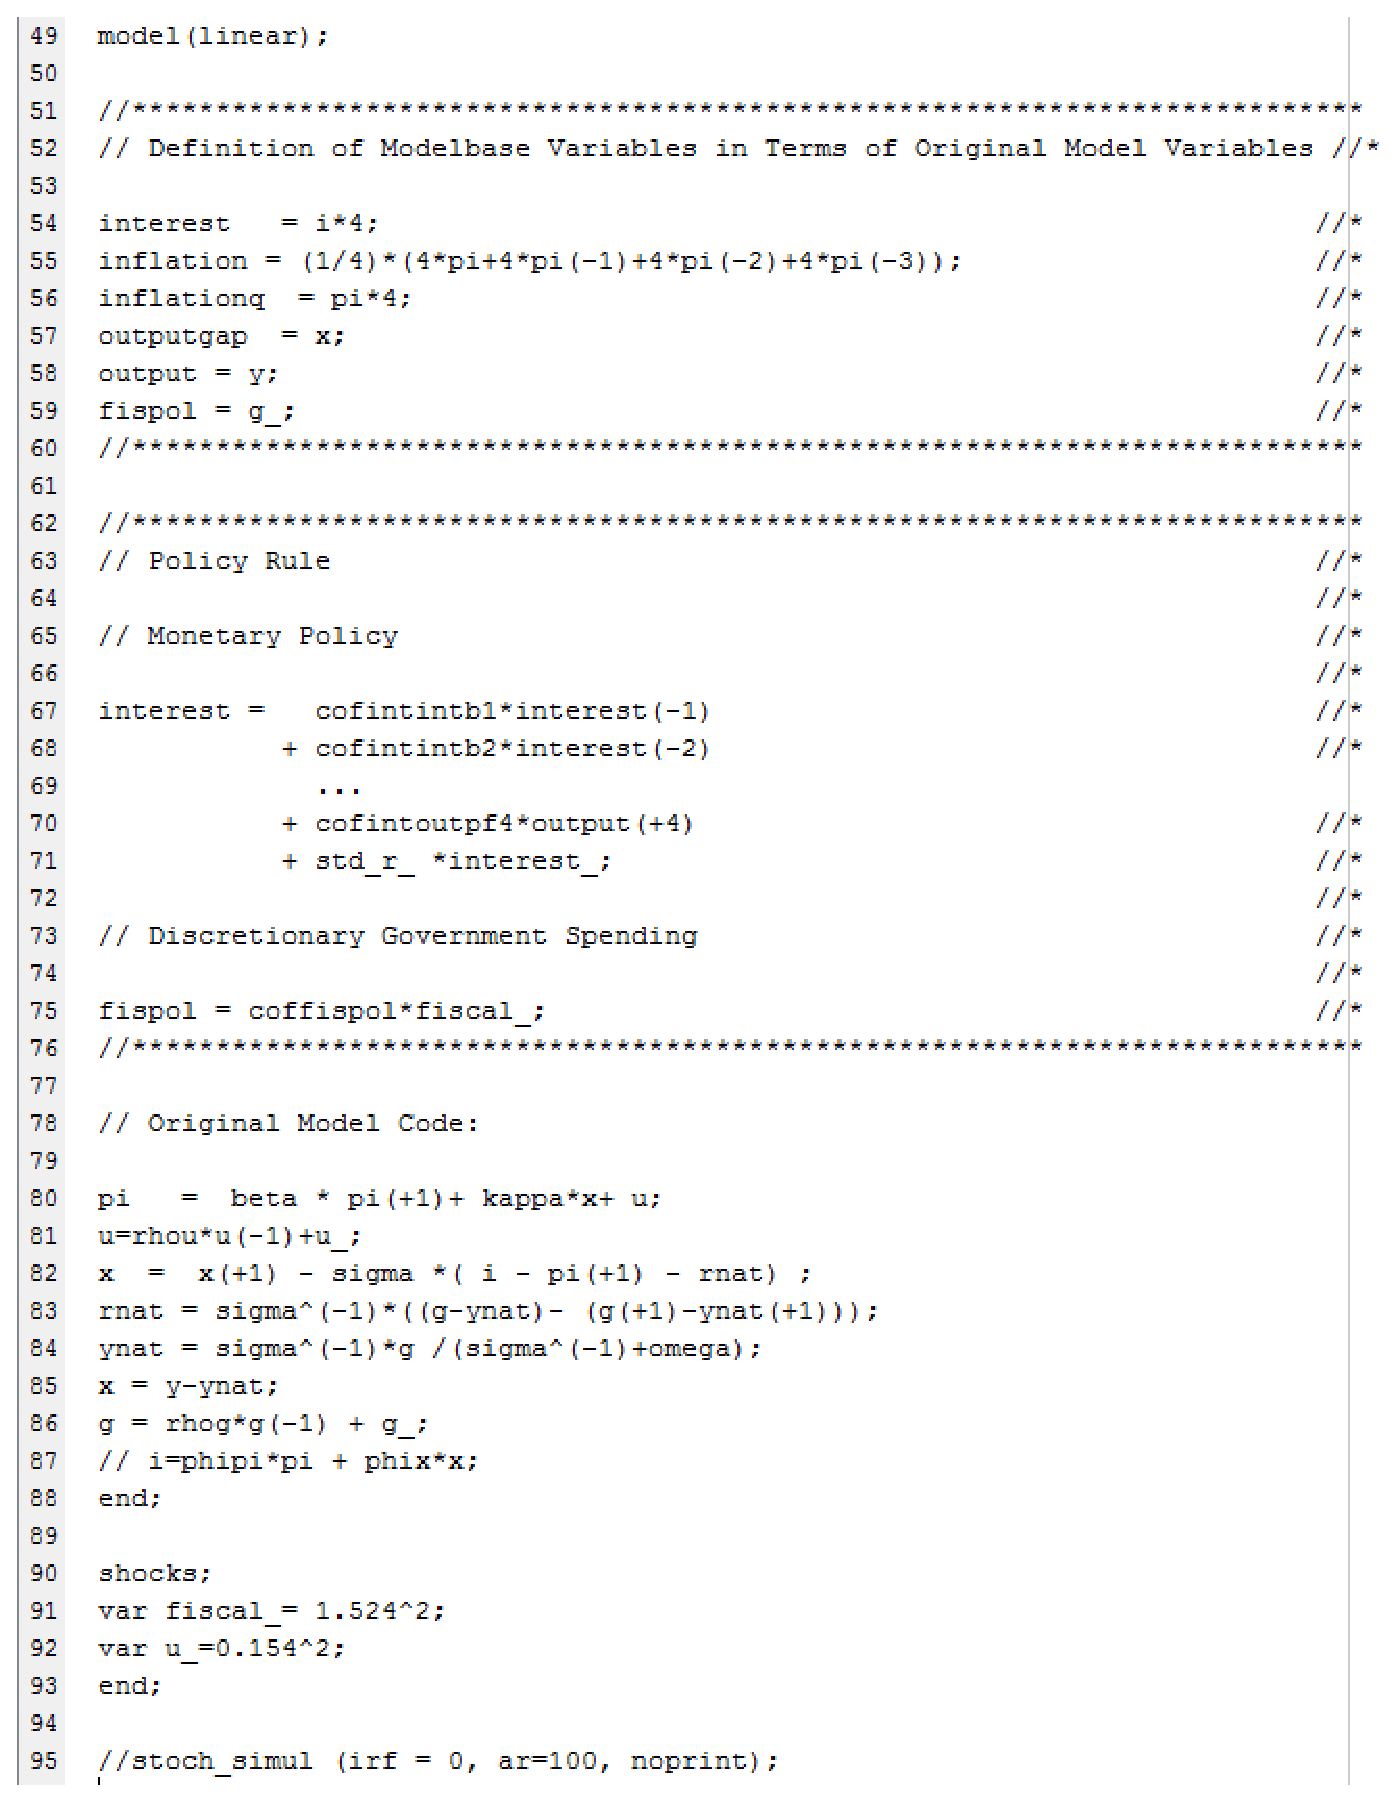
\includegraphics[width=15cm,keepaspectratio]{modStructureRW97b.eps}\\
\label{img:modStructureRW97b}
\end{figure}

\vspace{2cm}

\noindent {\it Part 1: The preamble}

\begin{itemize}
    \item Each model file begins with some information about the model. This should include the
    title, the authors, the publication etc. In front
    of this description you will find the symbols \textit{//}, which denote a comment in DYNARE.
    \item The file then starts with the initialization of the model variables. In our example shown in {\bf Figure
    \ref{img:modStructureRW97a}} the model-specific endogenous variables are listed in line 3 after the keyword \textit{var}:
    \textit{pi}, \textit{y}, \textit{ynat}, \textit{rnat}, \textit{i}, \textit{x}, \textit{u}, \textit{g}
    and \textit{g\_}. The latter in fact represents an exogenous government spending shock, however it has to be
    initialized as endogenous variable for reasons that will be explained below.
    It follows a Modelbase block in lines 4 to 7 in which the common variables are introduced.
    In general, Modelbase blocks are separated through \textit{//*******} symbols from the rest of the file.
    \item Following the keyword \textit{varexo} in line 9 the exogenous variables are initialized.
    In our example this is \textit{u\_}, a cost push shock as well as the common interest rate shock, \textit{interest\_} and
    the common fiscal policy shock, \textit{fiscal\_} in line 12. Note that in some models with no treatment of government spending, the
    latter Modelbase shock may be left out.
    \item Following the keyword \textit{parameters} in line 15, the Modelbase parameters in the Modelbase block are initialized.
    In {\bf Figure \ref{img:modStructureRW97a}} line 19 we have, for brevity reasons, only included three policy parameters.
    In the actual mod-files there are many more leads and lags. These are the parameters of the
    general monetary policy function, except for the last one, \textit{coffispol},
    which enters the common discretionary government spending equation.
    \item Then the model-specific parameters are initialized in line 21.
    \item Afterwards numerical values are assigned to the model-specific parameters in lines 23 to 32.
    \item Finally a block called \textit{Specification of Modelbase Parameters} is added. First in lines 37 to 44 the numeric
    values of the parameters of the selected monetary policy rule are loaded.
    They are contained in the file \textit{policy\_param.mat} in the subfolder \textit{MODELS}.
    For models in which the original shocks are expressed in percent/100 the parameter \textit{std\_r\_} has to be reset to 100
    after the parameter-loading command. In our example this would have to be done in line 43. However, the shocks in this model are
    already expressed in percentage terms. Secondly, the discretionary fiscal policy parameter \textit{coffispol} is defined as a function
    of the model-specific parameters in order to obtain a government spending shock of one percent of GDP. The exact
    implementation of the common fiscal policy shock will be described below. In our example no adjustment is
    needed and hence \textit{coffispol} is set equal to one.
\end{itemize}


\noindent {\it Part 2: The model block}

\begin{itemize}
\item The model block starts in line 49 of {\bf Figure \ref{img:modStructureRW97b}} as indicated by the keyword \textit{model} followed
by \textit{linear}, which tells DYNARE that the equations are already linearized and thus reduces computing time.
\item In the Modelbase block going from lines 51 to 60 the common variables are defined in terms of the original model variables.
The variable \textit{interest} denotes the annualized short-term interest rate, \textit{inflation} is annual inflation,
\textit{inflationq} represents annualized quarterly inflation, \textit{outputgap} and \textit{output} denote the output gap and output, respectively.
The common variable \textit{fispol} represents discretionary fiscal policy. It is set equal to the model-specific government spending
shock variable, which in the case of our example is \textit{g\_}. Note again, that this model-specific shock has to be initialized
as an endogenous variable. This allows us the keep the original model equation for government spending unchanged.
\item It follows the common \textit{Policy Rule} block. In lines 65 to 71 the common monetary policy rule is specified.
Again for reasons of brevity we have not displayed the complete general policy rule in {\bf Figure \ref{img:modStructureRW97b}}.
Below in line 73, the common equation for discretionary government spending is specified.
\item The original model equations are then specified in lines 78 to 87. Note that the model-specific monetary policy rule is commented out because the common policy rule is introduced. On the contrary, the government spending equation in line 86 has remained unchanged.
The model section ends in line 88 with the required keyword \textit{end}.
\item Finally the variance covariance matrix is specified in lines 91 and 92 between the keywords \textit{shocks} and \textit{end}. Importantly, the variance of the original model-specific government spending shock has been assigned to the common fiscal policy shock variable \textit{fiscal\_}. Hence, the common shock \textit{fiscal\_} affects the fiscal policy variable \textit{fispol} through the common discretionary government spending expression in line 75 which is set equal to the model-specific government spending shock \textit{g\_} in line 59.
\item The \textit{stoch\_simul} command in line 96 is commented out. Alternatively one can also delete this command.
\end{itemize}